\documentclass[12pt]{article}
\usepackage{amsmath, amssymb, amsthm, enumerate, graphicx}
\usepackage[usenames,dvipsnames]{color}
\usepackage{bm}
\usepackage[colorlinks=true,urlcolor=blue]{hyperref}
\usepackage{geometry}
\geometry{margin=1in}
\usepackage{float}
\usepackage{graphics}
\setlength{\marginparwidth}{2.15cm}
\usepackage{booktabs}
\usepackage{enumitem}
\usepackage{epsfig}
\usepackage{setspace}
\usepackage{parskip}
\usepackage[normalem]{ulem}
\usepackage{tikz}
\usetikzlibrary{positioning, arrows, automata}
\usepackage{pgfplots}
\pgfplotsset{compat=newest}
\usepackage[font=scriptsize]{subcaption}
\usepackage{float}
\usepackage[]{algorithm2e}
\usepackage{environ}
\usepackage{bbm}
\usepackage{graphicx}
\usepackage{titling}
\usepackage{url}
\usepackage{xcolor}
\usepackage{lipsum}
\usepackage{lastpage}
\usepackage[colorlinks=true,urlcolor=blue]{hyperref}
\usepackage{multicol}
\usepackage{tabularx}
\usepackage{comment}
\usepackage[utf8]{inputenc}
\usepackage{amssymb}
\usepackage{setspace}
\usepackage{marvosym}
\usepackage{wrapfig}
\usepackage{datetime}
\usepackage[many]{tcolorbox}
\usepackage{array}
\usepackage{multirow}
\usepackage{wasysym}
\usepackage{cancel}
\usepackage{cprotect}
\usepackage{listings}
\usepackage{color}


\newcommand{\R}{\mathbb{R}}
\newcommand{\blackcircle}{\tikz\draw[black,fill=black] (0,0) circle (1ex);}
\renewcommand{\circle}{\tikz\draw[black] (0,0) circle (1ex);}

\newtcolorbox[]{solution}[1][]{%
    breakable,
    enhanced,
    colback=white,
    title=Solution,
    #1
}

% SOLUTION environment
\NewEnviron{soln}{
\leavevmode\color{red}\ignorespaces \textbf{Solution} \BODY }{}

% QUESTION AUTHORS environment
\NewEnviron{qauthor}{
\leavevmode\color{blue}\ignorespaces \textbf{Author} \BODY}{}

% SOLUTION environment
\NewEnviron{qlearningobjective}{
\leavevmode\color{blue}\ignorespaces \textbf{Learning Objective } \BODY }{}

% TO ONLY SHOW HOMEWORK QUESTIONS, include following (else comment out):
\RenewEnviron{soln}{}
\RenewEnviron{qauthor}{}
\RenewEnviron{qlearningobjective}{}


%\newcommand{\norm}[1]{\lVert #1 \rVert}
%\newcommand{\st}{\mathrm{s.t.}}

\makeatletter
\newcommand{\removelatexerror}{\let\@latex@error\@gobble}
\makeatother

\newcommand{\argmax}{\mathop{\mathrm{argmax}}}
\newcommand{\argmin}{\mathop{\mathrm{argmin}}}

%%%%%%%%%%%%%%%%%%%%%%%%%%%%%%%%%%%%%%%%%%%
% Custom Math                             %
%%%%%%%%%%%%%%%%%%%%%%%%%%%%%%%%%%%%%%%%%%%

%%%%%%%%%%%%%%%%%%%%%%%%%%%%%%%%%%%%%%%%%%
% Custom commands                        %
%%%%%%%%%%%%%%%%%%%%%%%%%%%%%%%%%%%%%%%%%%

\newcommand{\vc}[1]{\boldsymbol{#1}}
\newcommand{\adj}[1]{\frac{d J}{d #1}}
\newcommand{\chain}[2]{\adj{#2} = \adj{#1}\frac{d #1}{d #2}}

% mathcal
\newcommand{\Ac}{\mathcal{A}}
\newcommand{\Bc}{\mathcal{B}}
\newcommand{\Cc}{\mathcal{C}}
\newcommand{\Dc}{\mathcal{D}}
\newcommand{\Ec}{\mathcal{E}}
\newcommand{\Fc}{\mathcal{F}}
\newcommand{\Gc}{\mathcal{G}}
\newcommand{\Hc}{\mathcal{H}}
\newcommand{\Ic}{\mathcal{I}}
\newcommand{\Jc}{\mathcal{J}}
\newcommand{\Kc}{\mathcal{K}}
\newcommand{\Lc}{\mathcal{L}}
\newcommand{\Mc}{\mathcal{M}}
\newcommand{\Nc}{\mathcal{N}}
\newcommand{\Oc}{\mathcal{O}}
\newcommand{\Pc}{\mathcal{P}}
\newcommand{\Qc}{\mathcal{Q}}
\newcommand{\Rc}{\mathcal{R}}
\newcommand{\Sc}{\mathcal{S}}
\newcommand{\Tc}{\mathcal{T}}
\newcommand{\Uc}{\mathcal{U}}
\newcommand{\Vc}{\mathcal{V}}
\newcommand{\Wc}{\mathcal{W}}
\newcommand{\Xc}{\mathcal{X}}
\newcommand{\Yc}{\mathcal{Y}}
\newcommand{\Zc}{\mathcal{Z}}

% mathbb
\newcommand{\Ab}{\mathbb{A}}
\newcommand{\Bb}{\mathbb{B}}
\newcommand{\Cb}{\mathbb{C}}
\newcommand{\Db}{\mathbb{D}}
\newcommand{\Eb}{\mathbb{E}}
\newcommand{\Fb}{\mathbb{F}}
\newcommand{\Gb}{\mathbb{G}}
\newcommand{\Hb}{\mathbb{H}}
\newcommand{\Ib}{\mathbb{I}}
\newcommand{\Jb}{\mathbb{J}}
\newcommand{\Kb}{\mathbb{K}}
\newcommand{\Lb}{\mathbb{L}}
\newcommand{\Mb}{\mathbb{M}}
\newcommand{\Nb}{\mathbb{N}}
\newcommand{\Ob}{\mathbb{O}}
\newcommand{\Pb}{\mathbb{P}}
\newcommand{\Qb}{\mathbb{Q}}
\newcommand{\Rb}{\mathbb{R}}
\newcommand{\Sb}{\mathbb{S}}
\newcommand{\Tb}{\mathbb{T}}
\newcommand{\Ub}{\mathbb{U}}
\newcommand{\Vb}{\mathbb{V}}
\newcommand{\Wb}{\mathbb{W}}
\newcommand{\Xb}{\mathbb{X}}
\newcommand{\Yb}{\mathbb{Y}}
\newcommand{\Zb}{\mathbb{Z}}

% mathbf lowercase
\newcommand{\av}{\mathbf{a}}
\newcommand{\bv}{\mathbf{b}}
\newcommand{\cv}{\mathbf{c}}
\newcommand{\dv}{\mathbf{d}}
\newcommand{\ev}{\mathbf{e}}
\newcommand{\fv}{\mathbf{f}}
\newcommand{\gv}{\mathbf{g}}
\newcommand{\hv}{\mathbf{h}}
\newcommand{\iv}{\mathbf{i}}
\newcommand{\jv}{\mathbf{j}}
\newcommand{\kv}{\mathbf{k}}
\newcommand{\lv}{\mathbf{l}}
\newcommand{\mv}{\mathbf{m}}
\newcommand{\nv}{\mathbf{n}}
\newcommand{\ov}{\mathbf{o}}
\newcommand{\pv}{\mathbf{p}}
\newcommand{\qv}{\mathbf{q}}
\newcommand{\rv}{\mathbf{r}}
\newcommand{\sv}{\mathbf{s}}
\newcommand{\tv}{\mathbf{t}}
\newcommand{\uv}{\mathbf{u}}
\newcommand{\vv}{\mathbf{v}}
\newcommand{\wv}{\mathbf{w}}
\newcommand{\xv}{\mathbf{x}}
\newcommand{\yv}{\mathbf{y}}
\newcommand{\zv}{\mathbf{z}}

% mathbf uppercase
\newcommand{\Av}{\mathbf{A}}
\newcommand{\Bv}{\mathbf{B}}
\newcommand{\Cv}{\mathbf{C}}
\newcommand{\Dv}{\mathbf{D}}
\newcommand{\Ev}{\mathbf{E}}
\newcommand{\Fv}{\mathbf{F}}
\newcommand{\Gv}{\mathbf{G}}
\newcommand{\Hv}{\mathbf{H}}
\newcommand{\Iv}{\mathbf{I}}
\newcommand{\Jv}{\mathbf{J}}
\newcommand{\Kv}{\mathbf{K}}
\newcommand{\Lv}{\mathbf{L}}
\newcommand{\Mv}{\mathbf{M}}
\newcommand{\Nv}{\mathbf{N}}
\newcommand{\Ov}{\mathbf{O}}
\newcommand{\Pv}{\mathbf{P}}
\newcommand{\Qv}{\mathbf{Q}}
\newcommand{\Rv}{\mathbf{R}}
\newcommand{\Sv}{\mathbf{S}}
\newcommand{\Tv}{\mathbf{T}}
\newcommand{\Uv}{\mathbf{U}}
\newcommand{\Vv}{\mathbf{V}}
\newcommand{\Wv}{\mathbf{W}}
\newcommand{\Xv}{\mathbf{X}}
\newcommand{\Yv}{\mathbf{Y}}
\newcommand{\Zv}{\mathbf{Z}}

% bold greek lowercase
\newcommand{\alphav     }{\boldsymbol \alpha     }
\newcommand{\betav      }{\boldsymbol \beta      }
\newcommand{\gammav     }{\boldsymbol \gamma     }
\newcommand{\deltav     }{\boldsymbol \delta     }
\newcommand{\epsilonv   }{\boldsymbol \epsilon   }
\newcommand{\varepsilonv}{\boldsymbol \varepsilon}
\newcommand{\zetav      }{\boldsymbol \zeta      }
\newcommand{\etav       }{\boldsymbol \eta       }
\newcommand{\thetav     }{\boldsymbol \theta     }
\newcommand{\varthetav  }{\boldsymbol \vartheta  }
\newcommand{\iotav      }{\boldsymbol \iota      }
\newcommand{\kappav     }{\boldsymbol \kappa     }
\newcommand{\varkappav  }{\boldsymbol \varkappa  }
\newcommand{\lambdav    }{\boldsymbol \lambda    }
\newcommand{\muv        }{\boldsymbol \mu        }
\newcommand{\nuv        }{\boldsymbol \nu        }
\newcommand{\xiv        }{\boldsymbol \xi        }
\newcommand{\omicronv   }{\boldsymbol \omicron   }
\newcommand{\piv        }{\boldsymbol \pi        }
\newcommand{\varpiv     }{\boldsymbol \varpi     }
\newcommand{\rhov       }{\boldsymbol \rho       }
\newcommand{\varrhov    }{\boldsymbol \varrho    }
\newcommand{\sigmav     }{\boldsymbol \sigma     }
\newcommand{\varsigmav  }{\boldsymbol \varsigma  }
\newcommand{\tauv       }{\boldsymbol \tau       }
\newcommand{\upsilonv   }{\boldsymbol \upsilon   }
\newcommand{\phiv       }{\boldsymbol \phi       }
\newcommand{\varphiv    }{\boldsymbol \varphi    }
\newcommand{\chiv       }{\boldsymbol \chi       }
\newcommand{\psiv       }{\boldsymbol \psi       }
\newcommand{\omegav     }{\boldsymbol \omega     }

% bold greek uppercase
\newcommand{\Gammav     }{\boldsymbol \Gamma     }
\newcommand{\Deltav     }{\boldsymbol \Delta     }
\newcommand{\Thetav     }{\boldsymbol \Theta     }
\newcommand{\Lambdav    }{\boldsymbol \Lambda    }
\newcommand{\Xiv        }{\boldsymbol \Xi        }
\newcommand{\Piv        }{\boldsymbol \Pi        }
\newcommand{\Sigmav     }{\boldsymbol \Sigma     }
\newcommand{\Upsilonv   }{\boldsymbol \Upsilon   }
\newcommand{\Phiv       }{\boldsymbol \Phi       }
\newcommand{\Psiv       }{\boldsymbol \Psi       }
\newcommand{\Omegav     }{\boldsymbol \Omega     }


%%%%%%%%%%%%%%%%%%%%%%%%%%%%%%%%%%%%%%%%%%%
% Custom box for highlights               %
%%%%%%%%%%%%%%%%%%%%%%%%%%%%%%%%%%%%%%%%%%%

% Define box and box title style
\tikzstyle{mybox} = [fill=blue!10, very thick,
    rectangle, rounded corners, inner sep=1em, inner ysep=1em]

% \newcommand{\notebox}[1]{
% \begin{tikzpicture}
% \node [mybox] (box){%
%     \begin{minipage}{\textwidth}
%     #1
%     \end{minipage}
% };
% \end{tikzpicture}%
% }

\NewEnviron{notebox}{

\begin{tikzpicture}
\node [mybox] (box){
    \begin{minipage}{\textwidth}
        \BODY
    \end{minipage}
};
\end{tikzpicture}
}


\begin{document}
\section*{}
\begin{center}
  \centerline{\textsc{\LARGE  Homework 3}}
  \vspace{0.5em}
  \centerline{\textsc{\LARGE KNN, Perceptron, Linear Regression, Decision Trees}\footnote{Compiled on \today{} at \currenttime{}}}
  \vspace{1em}
  \textsc{\large 10-301/10-601 Introduction to Machine Learning (Spring 2019)} \\
  \vspace{0.5em}
  \url{piazza.com/cmu/fall2019/1030110601} \\
  \vspace{0.5em}
  \centerline{OUT: Wednesday, Sep 18th, 2019}
  %\today{} at \currenttime{}}}
  \vspace{0.5em}
  \centerline{DUE: Wednesday, Sep 25th, 2019, 11:59pm}
    \centerline{TAs: Brynn Edmunds, Lisa Hou, Yujia Chen, Ayushi Sood}
\end{center}


\section*{START HERE: Instructions}

\begin{notebox}
Homework 3 covers topics on KNN, perceptron, and linear regression. The homework includes multiple choice, True/False, and short answer questions. 
\end{notebox}

\begin{itemize}
\item \textbf{Collaboration policy:} Collaboration on solving the homework is allowed, after you have thought about the problems on your own. It is also OK to get clarification (but not solutions) from books or online resources, again after you have thought about the problems on your own. There are two requirements: first, cite your collaborators fully and completely (e.g., ``Jane explained to me what is asked in Question 2.1''). Second, write your solution {\em independently}: close the book and all of your notes, and send collaborators out of the room, so that the solution comes from you only.  See the Academic Integrity Section on the course site for more information: \url{http://www.cs.cmu.edu/~mgormley/courses/10601/about.html#7-academic-integrity-policies}

\item\textbf{Late Submission Policy:} See the late submission policy here: \url{http://www.cs.cmu.edu/~mgormley/courses/10601/about.html#6-general-policies}

\item\textbf{Submitting your work:} 

\begin{itemize}

\item \textbf{Gradescope:} For written problems such as short answer, multiple choice, derivations, proofs, or plots, we will be using Gradescope (\url{https://gradescope.com/}). Please use the provided template. Submissions can be handwritten onto the template, but should be labeled and clearly legible. If your writing is not legible, you will not be awarded marks. Alternatively, submissions can be written in LaTeX. Regrade requests can be made, however this gives the TA the opportunity to regrade your entire paper, meaning if additional mistakes are found then points will be deducted.
Each derivation/proof should be completed on a separate page. For short answer questions, you \textbf{should not} include your work in your solution.  If you include your work in your solutions, your assignment may not be graded correctly by our AI assisted grader. In addition, please tag the problems to the corresponding pages when submitting your work.

\end{itemize}

% \item \textbf{Materials:} Download from autolab the tar file (``Download handout"). The tar file will contain all the data that you will need in order to complete this assignment.

\end{itemize}

%Homework 9 will be on Gradescope, but will be "Canvas-style"- all problems will be multiple choice, select all that apply, or numerical answer. 

For multiple choice or select all that apply questions, shade in the box or circle in the template document corresponding to the correct answer(s) for each of the questions. For \LaTeX users, use $\blacksquare$ and \blackcircle  for shaded boxes and circles, and don't change anything else.


\clearpage

\section*{Instructions for Specific Problem Types}

For ``Select One" questions, please fill in the appropriate bubble completely:

\begin{quote}
\textbf{Select One:} Who taught this course?
\begin{list}{}
     \item\CIRCLE{} Matt Gormley
     \item\Circle{} Marie Curie
     \item\Circle{} Noam Chomsky
\end{list}
\end{quote}

If you need to change your answer, you may cross out the previous answer and bubble in the new answer:

\begin{quote}
\textbf{Select One:} Who taught this course?
\begin{list}{}
     \item\CIRCLE{} Matt Gormley
     \item\Circle{} Marie Curie\\
     \xcancel{\CIRCLE}{} Noam Chomsky
\end{list}
\end{quote}


For ``Select all that apply" questions, please fill in all appropriate squares completely:

\begin{quote}
\textbf{Select all that apply:} Which are scientists?
    \begin{list}{}
    \item $\blacksquare$ Stephen Hawking 
    \item $\blacksquare$ Albert Einstein
    \item $\blacksquare$ Isaac Newton
    \item $\square$ I don't know
\end{list}
\end{quote}

Again, if you need to change your answer, you may cross out the previous answer(s) and bubble in the new answer(s):

\begin{quote}
\textbf{Select all that apply:} Which are scientists?
    \begin{list}{}
    \item $\blacksquare$ Stephen Hawking 
    \item $\blacksquare$ Albert Einstein
    \item $\blacksquare$ Isaac Newton\\
    \xcancel{$\blacksquare$} I don't know
\end{list}
\end{quote}

For questions where you must fill in a blank, please make sure your final answer is fully included in the given space. You may cross out answers or parts of answers, but the final answer must still be within the given space.

\begin{quote}
\textbf{Fill in the blank:} What is the course number?

\begin{tcolorbox}[fit,height=1cm, width=4cm, blank, borderline={1pt}{-2pt},nobeforeafter]
    \begin{center}\huge10-601\end{center}
    \end{tcolorbox}\hspace{2cm}
    \begin{tcolorbox}[fit,height=1cm, width=4cm, blank, borderline={1pt}{-2pt},nobeforeafter]
    \begin{center}\huge10-\xcancel{7}601\end{center}
    \end{tcolorbox}
\end{quote}


%\section*{Written Assignment [100 pts]}

\section{Decision Tree (Revisited) [9 pts]}


\begin{enumerate}

    \item \textbf{[2pt]} Suppose you are the 10-601 instructor trying to predict students' final exam grade using only homework grades. You decide to use historic records on this course to build a predictive model. However, someone messed up CMU's academic records system and the only information you have on students from past semesters is (i) if a student has submitted all homework (ii) if a student has attained maximum score on any of the homework (iii) if a student has scored 0 on any of the homework and  (iv) the students' letter grades on their final exams (this is the target, not attribute). You decide to use Decision Tree model, and since the information is so limited, you are satisfied as long as your model can predict the letter grade on the final exams  (A+, A, A-, B+, B, B-, C+, C and C-). Suppose that you have designed the grading policy to be percentile-based so all letter grades will show up. \\ \\
    Given enough past records and enough luck, will your model be able to do a perfect job (i.e., make no mistakes on students' letter grades of current semester)?
    
    \begin{list}{}
        \item $\circle$ Yes
        \item $\circle$ No
    \end{list}
    Why or why not? Explain your reason briefly (you can use mathematical expressions).\\
    
    \textbf{NOTE: Please do not change the size of the following text box, and keep your answer in it. Thank you!} \\ \\
    \begin{tcolorbox}[fit,height=2cm, width=15cm, blank, borderline={1pt}{-2pt},nobeforeafter]
    \large
    Your answer.

    \end{tcolorbox} \\
    
    \newpage
    \item \textbf{[2pt]} Consider the following $4\times 4$ checkerboard pattern. 
    \begin{figure}[H]
        \centering
        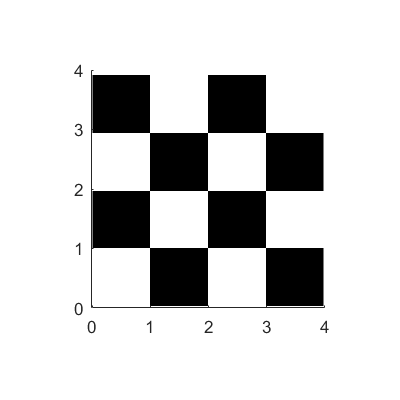
\includegraphics[width = 0.5\textwidth]{checkerboard.png}
        \label{Q_2dt}
    \end{figure}
    \begin{enumerate}
        \item What is the minimum depth of decision tree that perfectly classifies the $4\times 4$ colored regions, using $x$ and $y$ coordinates as separate features (how you use each of them is up to you)?
    \begin{list}{}
        \item $\circle$ 1
        \item $\circle$ 2
        \item $\circle$ 4
        \item $\circle$ 16
    \end{list}
    \item What is the minimum depth of decision trees to perfectly classify the colored regions, using ANY features?
    \begin{list}{}
        \item $\circle$ 1
        \item $\circle$ 2
        \item $\circle$ 4
        \item $\circle$ 16
    \end{list}
    \end{enumerate}
    
    \item \textbf{[3pt] Ensemble of Decision Tree.} Say we have a data set shown below. In total, there are 12 data points, with 6 in label "-" and 6 in label "+". We would like to use Decision Tree to solve this binary classification problem. However, in our problem setting, each Decision Tree has access to only ONE line. That is to say, our Decision Tree would have access to only one attribute, and so has max-depth of 1. \\ \\
    By accessing this line, the Decision Tree could know (and only know) whether the data point is on the right side of this line or the left side. (Unofficial definition: let's assume the right side of a line shares the same direction with the \textcolor{OliveGreen}{\textbf{green}} normal vector of that line.) \\ \\
    Finally, please use majority vote strategy to make classification decision at each leaf.\\
    
    \begin{figure}[H]
        \centering
        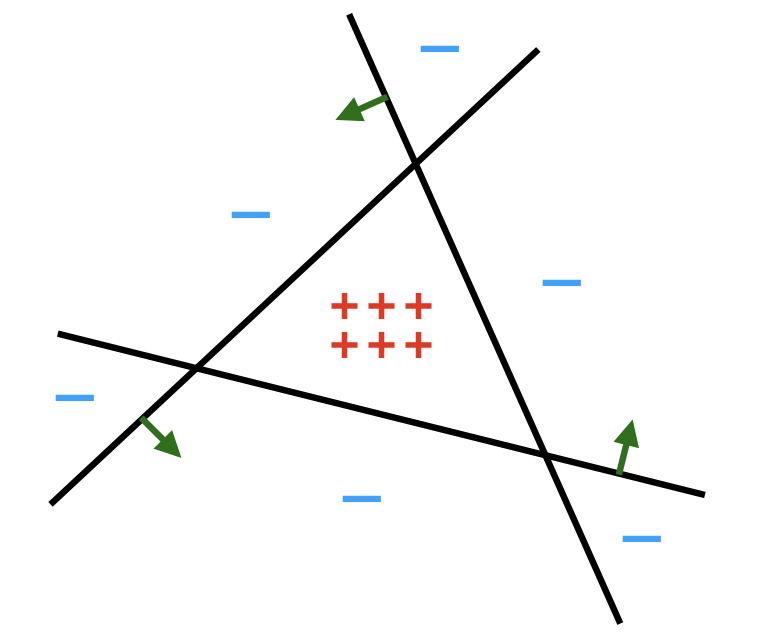
\includegraphics[width = 0.5\textwidth]{ensemble_dt.png}
        \label{Q_ensemble_DT}
    \end{figure}
    
    \begin{enumerate}
        \item  If we train only one Decision Tree, what is the best/lowest error rate? Note that we have in total 12 data points. (Please round to 4 decimal.) \\ \\
    \begin{tcolorbox}[fit,height=1cm, width=15cm, blank, borderline={1pt}{-2pt}, nobeforeafter]
    %solution
    \end{tcolorbox} 
    
    

    \item If we could use two Decision Trees, what is the best/lowest error rate? Let's say, if we have two Decision Trees, then each would predict each data point with label like '+' or '-'. Then we would like to combine these predictions as the final result. If these two all predict '+', then the result is '+'. The same with '-'. However, if one predicts '+' while one predicts '-', then to break tie, we always choose '-' as the final result. (Please round to 4 decimal.) \\ \\
    \begin{tcolorbox}[fit,height=1cm, width=15cm, blank, borderline={1pt}{-2pt}, nobeforeafter]
    %solution
    \end{tcolorbox} \\
    
    

\newpage
    \item Now let's train three Decision Trees as a forest, what is the best/lowest error rate? The ensemble strategy is now unanimous voting. That is, if every Decision Tree agree, then the final result is positive. However, if one of them has a different answer from the other two, then we predict negative. That means, we train each DT individually, with each DT choose one unique line as its decision boundary. Each DT would try its best to achieve high accuracy. And, next, if all DTs agrees, then it will give positive label. (Please round to 4 decimal.) \\ \\
    \begin{tcolorbox}[fit,height=1cm, width=15cm, blank, borderline={1pt}{-2pt}, nobeforeafter]
    %solution
    \end{tcolorbox} \\
    
    \end{enumerate}
    
    \item \textbf{[2pt]} Consider a binary classification problem using $1$-nearest neighbors. We have $N$ 1-dimensional training points $x_1, x_2, \ldots x_N$ and corresponding labels $y_1, y_2, \ldots y_N$ with $x_i \in \mathbb{R}$ and $y_i \in \{0, 1\}$. Assume the points $x_1, x_2, \ldots x_N$ are in ascending order by value. If there are ties during the 1-NN algorithm, we break ties by choosing the label of the $x_i$ with lower value. Assume we are using the Euclidean distance metric. Is it possible to build a decision tree where the decision at each node takes the form of “$x \leq t$ or $x > t$”, where $t \in \mathbb{R}$ behaves exactly the same as the 1-nearest neighbor classifier?
    
    \begin{list}{}
        \item $\circle$ Yes
        \item $\circle$ No
    \end{list}
     If your answer is yes, please explain how you will construct the decision tree. If your answer is no, explain why it’s not possible.  \\
   
    \textbf{NOTE: Please do not change the size of the following text box, and keep your answer in it. Thank you!} \\ \\
    \begin{tcolorbox}[fit,height=4cm, width=15cm, blank, borderline={1pt}{-2pt},nobeforeafter]
    \large
    Your answer.

    \end{tcolorbox} \\
    
    

    

\end{enumerate}




\newpage
\section{K-Nearest Neighbors [29 pts]}


\begin{enumerate}
    \item \textbf{[3pt]} Consider the description of two objects below:
    
    \begin{table}[H]
        \centering
        \begin{tabular}{c c c}
             & \textbf{Object A} & \textbf{Object B} \\
            Feature 1 & 3 & 9.1 \\
            Feature 2 & 2.1 & 0.7 \\
            Feature 3 & 4.8 & 2.2 \\
            Feature 4 & 5.1 & 5.1 \\
            Feature 5 & 6.2 & 1.8 
        \end{tabular}
    \end{table}
    We can reason about these objects as points in high dimensional space.
    
    Consider the two different distance functions below. Under which scheme are they closer in 5-D space?
    \begin{enumerate}
        \item Euclidean Distance: $d(x,y) = \sqrt{\sum_{i-1}^n (x_i - y_i)^2}$
        \item Manhattan Distance: $d(x,y) = \sum_{i=1}^n |x_i - y_i|$
    \end{enumerate}
    
    \textbf{Select one:}
    \begin{list}{}
        \item $\circle$ Euclidean Distance
        \item $\circle$ Manhattan Distance
    \end{list}

    
    
    \begin{figure}[H]
        \centering
        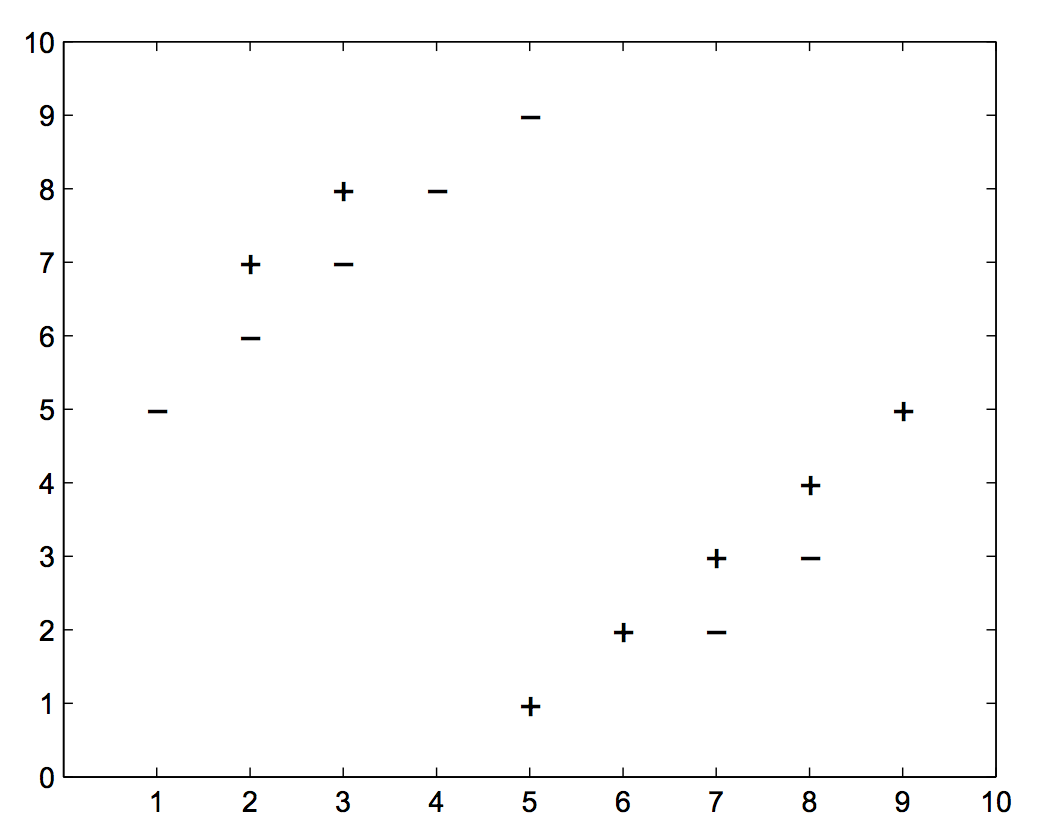
\includegraphics[width = 0.6\textwidth]{Q2_knn.png}
        \label{Q2_knn}
    \end{figure}

    \item \textbf{[3pt]} Consider a $k$-nearest neighbors binary classifier which assigns the class of a test point to be the class of the majority of the $k$-nearest neighbors, according to a Euclidean distance metric. Using the data set shown above to train the classifier and choosing $k=5$, which is the classification error on the training set? Assume that a point can be its own neighbor.
    
    Answer as a decimal with precision 4, e.g. (6.051, 0.1230, 1.234e+7)
    
    \begin{tcolorbox}[fit,height=1cm, width=4cm, blank, borderline={1pt}{-2pt},nobeforeafter]
    %solution
    \end{tcolorbox}
 
    
    
    \item \textbf{[3pt]} In the data set shown above, what is the value of $k$ that minimizes the training error? Note that a point can be its own neighbor. Let’s assume we use random-picking as the tie-breaking algorithm.
    
    \begin{tcolorbox}[fit,height=1cm, width=4cm, blank, borderline={1pt}{-2pt},nobeforeafter]
    %solution
    \end{tcolorbox}

    
    
    \item \textbf{[3pt]} Assume we have a training set and a test set drawn from the same distribution, and we would like to classify points in the test set using a $k$-NN classifier. 
    
    \begin{enumerate}
        \item In order to minimize the classification error on this test set, we should always choose the value of $k$ which minimizes the training set error. 
    
    \textbf{Select one:}
    \begin{list}{}
        \item $\circle$ True
        \item $\circle$ False
    \end{list}
    
    \item Instead of choosing the hyper-parameters by merely minimizing the training set error, some people would like to split the training-all data set into training and validation data set, and choose the hyper-parameters that lead to lower validation error. How do you think of this method? Justify your opinion with no more than 3 sentences.

    \textbf{Select one:}
    \begin{list}{}
        \item $\circle$ Good
        \item $\circle$ No good
    \end{list}

    \textbf{NOTE: Please do not change the size of the following text box, and keep your answer in it. Thank you!} \\ \\
    \begin{tcolorbox}[fit,height=4cm, width=15cm, blank, borderline={1pt}{-2pt},nobeforeafter]
    \large
    Your answer.

    \end{tcolorbox} \\

    \end{enumerate}
    
    
    \item \textbf{[3pt]} Consider a binary $k$-NN classifier where $k=4$ and the two labels are ``triangle" and ``square".
    
    Consider classifying a new point $\xv =(1,1)$, where two of the $\xv$'s nearest neighbors are labeled ``triangle" and two are labeled ``square" as shown below.
    
    \begin{figure}[H]
        \centering
        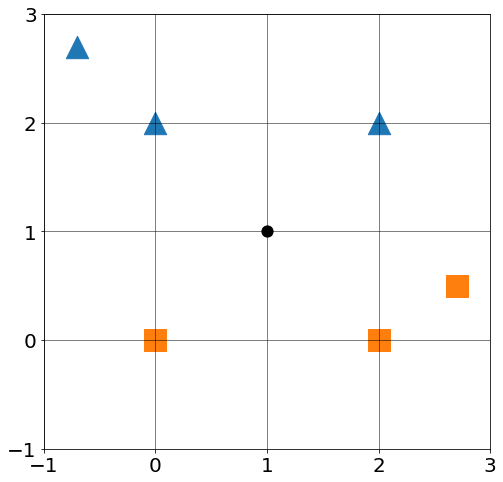
\includegraphics[width = 0.5\textwidth]{1-1-5.png}
        \label{Q_5knn}
    \end{figure}
    
    Which of the following methods can be used to break ties or avoid ties on this dataset?
    
    \begin{enumerate}
        \item Assign x the label of its nearest neighbor
        \item Flip a coin to randomly assign a label to $\xv$ (from the labels of its 4 closest points)
        \item Use $k = 3$ instead
        \item Use $k = 5$ instead
    \end{enumerate}

    \textbf{Select one:}
    \begin{list}{}
        \item $\circle$ a only
        \item $\circle$ b only
        \item $\circle$ b,c,d
        \item $\circle$ b,d
        \item $\circle$ d only
        \item $\circle$ a,b,c,d
        \item $\circle$ None of the above
    \end{list}
    
 
    
    \newpage
    \item \textbf{[2pt]} Consider the following data concerning the relationship between academic performance and salary after graduation. High school GPA and university GPA are two numerical variables (predictors) and salary is the numerical target. Note that salary is measured in thousands of dollars per year.
    
    \begin{table}[H]
        \centering
        \begin{tabular}{cccc}
            \textbf{Student ID} & \textbf{High School GPA} & \textbf{University GPA} & \textbf{Salary} \\
            1 & 2.2 & 3.4 & 45 \\
            2 & 3.9 & 2.9 & 55 \\
            3 & 3.7 & 3.6 & 91 \\
            4 & 4.0 & 4.0 & 142 \\
            5 & 2.8 & 3.5 & 88 \\
            6 & 3.5 & 1.0 & 2600 \\
            7 & 3.8 & 4.0 & 163 \\
            8 & 3.1 & 2.5 & 67 \\
            9 & 3.5 & 3.6 & unknown \\
        \end{tabular}
        \label{tab:my_label}
    \end{table}
    
    Among Students 1 to 8, who is the nearest neighbor to Student 9, using Euclidean distance?
    
    Answer the Student ID only.

    \begin{tcolorbox}[fit,height=1cm, width=4cm, blank, borderline={1pt}{-2pt},nobeforeafter]
    %solution
    \end{tcolorbox}

 
    
    
    \item \textbf{[3pt]} In the data set shown above, our task is to predict the salary Student 9 earns after graduation. We apply $k$-NN to this regression problem: the prediction for the numerical target (salary in this example) is equal to the average of salaries for the top $k$ nearest neighbors. 
    
    If $k=3$, what is our prediction for Student 9's salary?
    
    Round your answer to the nearest integer. Be sure to use the same unit of measure (thousands of dollars per year) as the table above.
    
    \begin{tcolorbox}[fit,height=1cm, width=4cm, blank, borderline={1pt}{-2pt},nobeforeafter]
    %solution
    \end{tcolorbox}
    
    

\newpage
    \item \textbf{[3pt]} Suppose that the first 8 students shown above are only a subset of your full training data set, which consists of 10,000 students. We apply KNN regression using Euclidean distance to this problem and we define training loss on this full data set to be the mean squared error (MSE) of salary.

    Now consider the possible consequences of modifying the data in various ways. Which of the following changes \textbf{could} have an effect on training loss on the full data set as measured by mean squared error (MSE) of salary? Select all that apply.
    
    
        
    \textbf{Select all that apply:}
    \begin{list}{}
        \item $\square$ Rescaling only ``High School GPA" to be a percentage of 4.0
        \item $\square$ Rescaling only ``University GPA" to be a percentage of 4.0
        \item $\square$ Rescaling both ``High School GPA" and ``University GPA", so that each is a percentage of 4.0 (scale by the same percentage).
        \item $\square$ None of the above.
    \end{list}

    
    
    \item \textbf{[3pt]} In this question, we would like to compare the differences among KNN, the perceptron algorithm, and linear regression. Please select all that apply.
    
    \textbf{Select all that apply:}
    \begin{list}{}
        \item $\square$ For classification tasks, both KNN and the perceptron algorithm can have linear decision boundaries.
        \item $\square$ For classification tasks, both KNN and the perceptron algorithm always have linear decision boundaries.
        \item $\square$ All three models can be susceptible to overfitting.
        \item $\square$ In all three models, after the training is completed, we must store the training data to make predictions on the test data.
        \item $\square$ None of the above.
    \end{list}

    

    \item \textbf{[3pt]} Please select all that apply about kNN in the following options.

    \textbf{Select all that apply:}
    \begin{list}{}
        \item $\square$ Large $k$ gives a smoother decision boundary
        \item $\square$ To reduce the impact of noise or outliers in our data, we should increase the value $k$.
        \item $\square$ If we make $k$ too large, we could end up overfitting the data.
        \item $\square$ We can use cross-validation to help us select the value of $k$.
        \item $\square$ We should never select the $k$ that minimizes the error on the validation dataset.
        \item $\square$ None of the above.
    \end{list}

    
    
    \clearpage
\end{enumerate}

\section{Perceptron [22 pts]}
\begin{enumerate}
    \item \textbf{[2pt]} Consider running the online perceptron algorithm on some sequence of examples $S$ (an example is a data point and its label). Let $S^\prime$ be the same set of examples as $S$, but presented in a different order.
    
    True or False: the online perceptron algorithm is guaranteed to make the same number of mistakes on $S$ as it does on $S^\prime$.

    \textbf{Select one:}
    \begin{list}{}
        \item $\circle$ True
        \item $\circle$ False
    \end{list}


    
    \item \textbf{[3pt]} Suppose we have a perceptron whose inputs are 2-dimensional vectors and each feature vector component is either 0 or 1, i.e., $x_i \in \{0,1\}$. The prediction function $y = \operatorname{sign}(w_1x_1 + w_2x_2 + b)$, and
    $$
    \operatorname{sign}(z) = 
    \begin{cases}
    1, & \textrm{ if } z \geq 0\\
    0, & \textrm{ otherwise}.
    \end{cases}
    $$
    Which of the following functions can be implemented with the above perceptron? That is, for which of the following functions does there exist a set of parameters $w,b$ that correctly define the function. Select all that apply.
    
    \textbf{Select all that apply:}
    \begin{list}{}
        \item $\square$ AND function, i.e., the function that evaluates to 1 if and only if all inputs are 1, and 0 otherwise.
        \item $\square$ OR function, i.e., the function that evaluates to 1 if and only if at least one of the inputs are 1, and 0 otherwise.
        \item $\square$ XOR function, i.e., the function that evaluates to 1 if and only if the inputs are not all the same. For example
        $$
        \operatorname{XOR}(1,0) = 1, \textrm{ but } \operatorname{XOR}(1,1) = 0.
        $$
        \item $\square$ None of the above.
    \end{list}

    
    
    \clearpage
    
    \item \textbf{[2pt]} Suppose we have a dataset $\left\{ \left(\xv^{(1)},y^{(1)}\right),\ldots, \left(\xv^{(N)},y^{(N)}\right) \right\}$, where $\xv^{(i)} \in \mathbb{R}^M$, $y^{(i)}\in\{+1,-1\}$. We would like to apply the perceptron algorithm on this dataset. Assume there is no intercept term. How many parameter values is the perceptron algorithm learning?

    \textbf{Select one:}
    \begin{list}{}
        \item $\circle$ $N$
        \item $\circle$ $N\times M$
        \item $\circle$ $M$
    \end{list}


    
    \item \textbf{[3pt]} Which of the following are true about the perceptron algorithm? Select all that apply.

    \textbf{Select all that apply:}
    \begin{list}{}
        \item $\square$ The number of mistakes the perceptron algorithm makes is proportional to the size of the dataset. 
        \item $\square$ The perceptron algorithm converges on any dataset.
        \item $\square$ The perceptron algorithm can be used in the context of online learning.
        \item $\square$ For linearly spearable data, the perceptron algorithm always finds the separating hyperplane with the largest margin.
        \item $\square$ None of the above.
    \end{list}

    
    
    \item \textbf{[3pt]} Suppose we have the following data:     \begin{align*}
        \xv^{(1)} &= [1,2] & \xv^{(2)} &= [-1,2] & \xv^{(3)} &= [-2,3] & \xv^{(4)} &= [1,-1] \\
        y^{(1)} &= 1 & y^{(2)} &= -1 & y^{(3)} &= -1 & y^{(4)} &= 1
    \end{align*}
    Starting from $\wv = [0,0]$, what is the vector $\wv$ after running the perceptron algorithm with exactly one pass over the data (pass= one iteration of the algorithm, going through all datapoints)? Assume we are running the perceptron algorithm without an intercept term. If the value of the dot product of a data point and the weight vector is $0$, the algorithm makes the prediction 1.

    \textbf{Select one:}
    \begin{list}{}
        \item $\circle$ $[1,-2]$
        \item $\circle$ $[2,0]$
        \item $\circle$ $[-1,1]$
        \item $\circle$ $[1,-3]$
    \end{list}

    
    
    \clearpage

    \item \textbf{[2pt]} Please refer to previous question for the data. Assume we are running perceptron in the batch setting. How many passes will the perceptron algorithm make before converging to a perfect classifier, i.e., one that does not make any false predictions on this dataset?

    \textbf{Select one:}
    \begin{list}{}
        \item $\circle$ $2$
        \item $\circle$ $3$
        \item $\circle$ $5$
        \item $\circle$ Infinitely many (the algorithm does not converge)
    \end{list}

    
    
        
    % \clearpage
    
    \item \textbf{[3pt]} Please select the correct statement(s) about the mistake bound of the perceptron algorithm. Select all that apply.

    \textbf{Select all that apply:}
    \begin{list}{}
        \item $\square$ If the minimum distance from any data point to the separating hyperplane is increased, without any other change to the data points, the mistake bound will also increase.
        \item $\square$ If the whole dataset is shifted away from origin, then the mistake bound will also increase.
        \item $\square$ If the size of the data set (i.e., the maximum pair-wise distance between data points) is increased, then the mistake bound will also increase.
        \item $\square$ The mistake bound is linearly inverse-proportional to the minimum distance of any data point to the separating hyperplane of the data.
        \item $\square$ None of the above.
    \end{list}



    \item \textbf{[2pt]} Given a zero-centered 3-dimensional dataset, the coordinate of the point with the highest L-2 norm is $(2, 2, 2)$. Assuming that the dataset is linearly separable with margin 2, what is the greatest number of mistakes that Perceptron could make?

    \textbf{Select one:}
    \begin{list}{}
        \item $\circle$ $1$
        \item $\circle$ $2$
        \item $\circle$ $3$
        \item $\circle$ $4$
    \end{list}

\newpage
    \item \textbf{[2pt]} Suppose we have data whose elements are of the form $[x_1,x_2]$, where $x_1 - x_2 = 0$. We do not know the label for each element. Suppose the perceptron algorithm starts with $\bm{\theta} = [3,5]$, which of the following values will $\bm{\theta}$ never take on in the process of running the perceptron algorithm on the data?

    \textbf{Select one:}
    \begin{list}{}
        \item $\circle$ $[-1,1]$
        \item $\circle$ $[4,6]$
        \item $\circle$ $[-3,-1]$
        \item $\circle$ $[5,5]$
    \end{list}


    
    

    
    

    \clearpage
\end{enumerate}

\section{Linear Regression [40 pts]}
\begin{enumerate}

    \item \textbf{[4pt]} Suppose you have data ${(x^{(1)}, y^{(1)}), \ldots, (x^{(n)}, y^{(n)})}$ and the solution to linear regression on this data is $y = w_1 x + b_1$. Now suppose we have the dataset \\
    ${(x^{(1)} + \alpha, y^{(1)} + \beta), \ldots, (x^{(n)} + \alpha, y^{(n)} + \beta)}$ where $\alpha > 0, \beta > 0$ and $w_1 \alpha \neq \beta$. The solution to the linear regression on this dataset is $y = w_2 x + b_2$. Please select the correct statement about $w_1, w_2, b_1, b_2$ below. Note that the statement should hold no matter what values $\alpha, \beta$ take on within the specified constraints.
    
    \textbf{Select one:}
    \begin{list}{}
        \item $\circle$ $w_1 = w_2, b_1 = b_2$
        \item $\circle$ $w_1 \neq w_2, b_1 = b_2$
        \item $\circle$ $w_1 = w_2, b_1 \neq b_2$
        \item $\circle$ $w_1 \neq w_2, b_1 \neq b_2$
    \end{list}
    

    \item \textbf{[4pt]} We would like to fit a linear regression estimate to the dataset 
    $$
    D = \left\{\left(\xv^{(1)},y^{(1)}\right), \left(\xv^{(2)},y^{(2)}\right),\cdots, \left(\xv^{(N)},y^{(N)}\right)\right\}
    $$ with $\xv^{(i)} \in \mathbb{R}^M$ by minimizing the ordinary least square (OLS) objective function:
    $$
    J(\wv) = \frac{1}{2}\sum_{i=1}^N\left(y^{(i)} - \sum_{j=1}^M w_j x_j^{(i)}\right)^2
    $$
    Specifically, we solve for each coefficient $w_k$ ($1\leq k\leq M$) by deriving an expression of $w_k$ from the critical point $\frac{\partial J(\wv)}{\partial w_k} = 0$. What is the expression for each $w_k$ in terms of the dataset $(\xv^{(1)},y^{(1)}), (\xv^{(2)},y^{(2)}),\cdots, (\xv^{(N)},y^{(N)})$ and $w_1,\cdots,w_{k-1},w_{k+1},\cdots,w_M$?

    \textbf{Select one:}
    \begin{list}{}
        \item $\circle$ $w_k = \frac{\sum_{i=1}^N x_k^{(i)}(y^{(i)}-\sum_{j=1,j\neq k}^M w_j x_j^{(i)})}{\sum_{i=1}^N (x_k^{(i)})^2}$
        \item $\circle$ $w_k = \frac{\sum_{i=1}^N x_k^{(i)}(y^{(i)}-\sum_{j=1,j\neq k}^M w_j x_j^{(i)})}{\sum_{i=1}^N (y^{(i)})^2}$
        \item $\circle$ $w_k = \sum_{i=1}^N x_k^{(i)}(y^{(i)}-\sum_{j=1}^M w_j x_j^{(i)})$
        \item $\circle$ $w_k = \frac{\sum_{i=1}^N x_k^{(i)}(y^{(i)}-\sum_{j=1,j\neq k}^M w_j x_j^{(i)})}{\sum_{i=1}^N (x_k^{(i)} y^{(i)})^2}$
    \end{list}

    
    
    \clearpage
    
    \item \textbf{[3pt]} Continuing from the above question, how many coefficients do you need to estimate? When solving for these coefficients, how many equations do you have?
    
    \textbf{Select one:}
    \begin{list}{}
        \item $\circle$ $N$ coefficients, $M$ equations
        \item $\circle$ $M$ coefficients, $N$ equations
        \item $\circle$ $M$ coefficients, $M$ equations
        \item $\circle$ $N$ coefficients, $N$ equations
    \end{list}
    
    
    \item \textbf{[3pt]} Consider the following 3 data points for linear regression: $x^{(1)} = [0, 1, 2]^T$, $x^{(2)} = [1, 0, 2]^T$ and $x^{(3)} = [2, 1, 0]^T$. The corresponding y values are $y^{(1)}=3$, $y^{(2)}=6$, $y^{(3)}=9$.
    
    Assume the intercept to be 0. Find the weights $\theta = [\theta_1,  \theta_2,  \theta_3]^T \in \mathbb{R}^3$ such that the mean squared error $J(\theta) = (\textbf{y} - X\theta)^T(\textbf{y} - X\theta)$ is minimized on this training set. $X$ is the design matrix where $X_{ij} = x_j^{(i)}$. 
    
    $\theta_1$: \quad
    \begin{tcolorbox}[fit,height=1cm, width=4cm, blank, borderline={1pt}{-2pt},nobeforeafter]
    \end{tcolorbox}
    
    
    $\theta_2$: \quad
    \begin{tcolorbox}[fit,height=1cm, width=4cm, blank, borderline={1pt}{-2pt},nobeforeafter]
    \end{tcolorbox}
    
    
    $\theta_3$: \quad
    \begin{tcolorbox}[fit,height=1cm, width=4cm, blank, borderline={1pt}{-2pt},nobeforeafter]
    \end{tcolorbox}
    
    

    \item \textbf{[1pt]} Suppose we are working with datasets where the number of features is 3. The optimal solution for linear regression is always unique regardless of the number of data points that are in this dataset.
    
    \textbf{Select one:}
    \begin{list}{}
        \item $\circle$ True
        \item $\circle$ False
    \end{list}
    
    
    \item \textbf{[1pt]} Assume that a data set has $M$ data points and $N$ variables, where $M>N$. As long as we use a convex loss function, the regression problem will return the same set of solutions.
    
    \textbf{Select one:}
    \begin{list}{}
        \item $\circle$ True
        \item $\circle$ False
    \end{list}
    
    
    \newpage
    \item \textbf{[1pt]} Consider the following dataset:
        \begin{table}[H]
    \centering
        \begin{tabular}{llllll}
        x & 1.0 & 2.0 & 3.0 & 4.0 & 5.0 \\
        z & 2.0 & 4.0 & 6.0 & 8.0 & 10.0 \\
        y & 4.0 & 7.0 & 8.0 & 11.0 & 17.0
        \end{tabular}
    \end{table}
   We want to carry out a multiple-linear regression between $y$ (Dependent Variable) and $x$ and $z$ (Independent Variables). The closed-form solution given by $\wv = \left(\Xv^T\Xv\right)^{-1}\Xv^T Y$ will return the unique solution. 
    \\~\\
    Note: The $i^{th}$ row of $\Xv$ contains the $i^{th}$ data point $(x_i,z_i)$ while the $i^{th}$ row of $\Yv$ contains the $i^{th}$ data point $y_i$. 
    
        \textbf{Select one:}
    \begin{list}{}
        \item $\circle$ True
        \item $\circle$ False
    \end{list}
    

    
    \item \textbf{[3 pt]} Order the following different formulations of the regression cost function according to sensitivity to outliers from the most sensitive to the least sensitive. 
\begin{enumerate}
    \item $J(\mathbf{w}) = \sum\limits_{i} | (x^i)^T\mathbf{w}-y^i|^2$
    \item $J(\mathbf{w}) = \sum\limits_{i} | (x^i)^T\mathbf{w}-y^i|^4$
    \item $J(\mathbf{w}) = \sum\limits_{i} | (x^i)^T\mathbf{w}-y^i|$
\end{enumerate}

\textbf{Order the cost functions here:}

    1: \quad
    \begin{tcolorbox}[fit,height=1cm, width=2cm, blank, borderline={1pt}{-2pt},nobeforeafter]
    \end{tcolorbox}
    
    
    2: \quad
    \begin{tcolorbox}[fit,height=1cm, width=2cm, blank, borderline={1pt}{-2pt},nobeforeafter]
    \end{tcolorbox}
    
    
    3: \quad
    \begin{tcolorbox}[fit,height=1cm, width=2cm, blank, borderline={1pt}{-2pt},nobeforeafter]
    \end{tcolorbox}
    
    
    \newpage
    \item \textbf{[2 pt]} Which of the following are true about regularization?
    \textbf{Select all that apply:}
    \begin{list}{}
        \item $\square$ One of the goals of regularization is combating overfitting.
        \item $\square$ A model with regularization fits the training data better than a model without regularization 
        \item $\square$ The L-0 norm (number of non-zero parameters) is rarely used in practice in part because it is non-differentiable. 
        \item $\square$ One way to understand regularization is that it attempts to follow Occam's razor and make the learning algorithm prefer "simpler" solutions.
    \end{list}
    
    \item \textbf{[3pt]} Identifying whether a function is a convex function is useful because a convex function's local minimum has the nice property that it has to be the global minimum. Please select all functions below that are convex functions. Note $dom(f)$ denotes the domain of the function $f$.
    
    \textbf{Select all that apply:}
    \begin{list}{}
        \item $\square$ $f(x) = x, dom(f) = \mathbb{R}$
        \item $\square$ $f(x) = x^3 + 2x + 3, dom(f) = \mathbb{R}$
        \item $\square$ $f(x) = \log x, dom(f) = \mathbb{R}_{++}$ (the set of positive real numbers)
        \item $\square$ $f(x) = |x|, dom(f) = \mathbb{R}$
        \item $\square$ $f(x) = ||\xv||_2,\, dom(f) = \mathbb{R}^n$
        \item $\square$ None of the above.
    \end{list}


    \item \textbf{[2pt]} Typically we can solve linear regression problems in two ways. One is through direct methods, e.g. solving the closed form solution, and the other is through iterative methods (gradient descent). Consider a linear regression on data $(\Xv, \yv)$. We assume each row in $\Xv$ denotes one input in the dataset. Please select all correct options.
    
    \textbf{Select all that apply:}
    \begin{list}{}
        \item $\square$ If the matrix $\Xv^T\Xv$ is invertible, the exact solution is always preferred for solving the solution to linear regression as computing matrix inversions and multiplications are fast regardless of the size of the dataset.
        \item $\square$ Assume $N$ is the number of examples and $M$ is the number of features. The computational complexity of $N$ iterations of batch gradient descent is $\mathcal{O}(MN)$.
        \item $\square$ The computational complexity of the closed form solution is linear in number of parameters/features.
        \item $\square$ None of the above.
    \end{list}
    
    
    
    \newpage
    \item \textbf{[3 pts]} When performing linear regression, which of the following options will decrease mean-squared training error:
    
    \textbf{Select all that apply:}
        \begin{list}{}
        \item $\square$ Increasing the order of the polynomial
        \item $\square$ Increasing the regularization weight
        \item $\square$ For the same weight on the regularizer, using an L1 regularizer instead of an L2
        \item $\square$ For the same weight on the regularizer, using an L1 regularizer instead of an L0
        \item $\square$ None of the above
        \end{list}


    
    \item \textbf{[2pt]} \label{Q7_linear_regression} Consider the following dataset:
    \begin{table}[H]
    \centering
        \begin{tabular}{llllll}
        x & 1.0 & 2.0 & 3.0 & 4.0 & 5.0 \\
        y & 3.0 & 8.0 & 9.0 & 12.0 & 15.0
        \end{tabular}
    \end{table}
    If we initialize the weight as $2.0$ and intercept as $0.0$, what is the gradient of the loss function with respect to the weight $w$, calculated over all the data points, in the first step of the gradient descent update? Note that we do not introduce any regularization in this problem and and our objective function looks like $\frac{1}{N}\sum_{i=1}^N (wx_i + b - y_i)^2$, where $N$ is the number of data points, $w$ is the weight, and $b$ is the intercept.
    
    Fill in the blank with the gradient on the weight you computed, rounded to 2 decimal places after the decimal point.
    
    \begin{tcolorbox}[fit,height=1cm, width=4cm, blank, borderline={1pt}{-2pt},nobeforeafter]
    \end{tcolorbox}
    
    
    
    \item \textbf{[4pt]} Based on the data of the previous question, please compute the direct solution of the weight and the intercept for the objective function defined in the previous question, rounded to 2 decimal places after the decimal point.
    
    Weight: \quad
    \begin{tcolorbox}[fit,height=1cm, width=4cm, blank, borderline={1pt}{-2pt},nobeforeafter]
    \end{tcolorbox}
    
    
    Intercept: \quad
    \begin{tcolorbox}[fit,height=1cm, width=4cm, blank, borderline={1pt}{-2pt},nobeforeafter]
    \end{tcolorbox}
    
    
    
    \newpage
    \item \textbf{[2pt]} Using the dataset and model given in question \ref{Q7_linear_regression}, perform two steps of batch gradient descent on the data. Fill in the blank with the value of the weight after two steps of batch gradient descent. Let the learning rate be $0.01$. Round to 2 decimal places after the decimal point.
    
    \begin{tcolorbox}[fit,height=1cm, width=4cm, blank, borderline={1pt}{-2pt},nobeforeafter]
    \end{tcolorbox}
    
    
    
    \item \textbf{[2pt]} Using the dataset and model given in question \ref{Q7_linear_regression}, which of the following learning rates leads to the most optimal weight and intercept after performing two steps of batch gradient descent? (Hint: The most optimal learned parameters are the parameters that lead to the lowest value of the objective function.)
    
    \textbf{Select one:}
    \begin{list}{}
        \item $\circle$ $1$
        \item $\circle$ $0.1$
        \item $\circle$ $0.01$
        \item $\circle$ $0.001$
    \end{list}
    
    
    

    \clearpage
\end{enumerate}




\clearpage


\begin{comment} 
{\bf Collaboration Questions} After you have completed all other components of this assignment, report your answers to the collaboration policy questions detailed in the Academic Integrity Policies found \href{http://www.cs.cmu.edu/~mgormley/courses/10601-s18/about.html#7-academic-integrity-policies}{here}.
    \begin{enumerate*}
        \item Did you receive any help whatsoever from anyone in solving this assignment? If so, include full details.
        \item Did you give any help whatsoever to anyone in solving this assignment? If so, include full details?
        \item Did you find or come across code that implements any part of this assignment ? If so, include full details.
    \end{enumerate*}
    
    \begin{tcolorbox}[fit,height=3cm,blank, borderline={1pt}{-2pt},nobeforeafter]
    %Input your solution here.  Do not change any of the specifications of this solution box.
    \end{tcolorbox}
\end{comment}


\textbf{Collaboration Questions} Please answer the following:


    After you have completed all other components of this assignment, report your answers to the collaboration policy questions detailed in the Academic Integrity Policies found \href{http://www.cs.cmu.edu/~mgormley/courses/10601/about.html#7-academic-integrity-policies}{here}.
    \begin{enumerate}
        \item Did you receive any help whatsoever from anyone in solving this assignment? Is so, include full details.
        \item Did you give any help whatsoever to anyone in solving this assignment? Is so, include full details.
        \item Did you find or come across code that implements any part of this assignment ? If so, include full details.
    \end{enumerate}
    
    \begin{solution}
    % If you are using the latex template, remove the empty spaces
    \bigskip \bigskip \bigskip \bigskip \bigskip \bigskip \bigskip \bigskip
    \bigskip \bigskip \bigskip \bigskip \bigskip \bigskip \bigskip \bigskip
    \bigskip \bigskip \bigskip \bigskip \bigskip \bigskip \bigskip \bigskip
    \bigskip \bigskip \bigskip \bigskip \bigskip \bigskip \bigskip \bigskip
    \bigskip \bigskip \bigskip \bigskip \bigskip \bigskip \bigskip \bigskip
    \bigskip \bigskip \bigskip \bigskip \bigskip \bigskip \bigskip \bigskip
    \bigskip \bigskip \bigskip \bigskip \bigskip \bigskip \bigskip \bigskip
    \end{solution}
    

\end{document}